% !Mode:: "TeX:UTF-8"

\chapter{预备知识}
\label{ch:pre}



\section{图像的视觉信息抽取}



\subsection{神经网络}

\subsubsection{一般神经网络}
神经网络(neural network)的方面的研究就出现了,早起的神经网络主要是指生物学中的``生物神经网络'',在当前计算机领域特指``神经网络学习''。神经网络最基本的结构是神经元模型,神经元模型如图\ref{fig:nn-example},在这个模型中包括输入端、神经元权重(weight)、偏差(bias)、激活函数(activation function)、阀值、输出。在这个模型中,当前神经元接收其它$n$个神经元的输入,与连接权重相乘之后加上偏差,然后激活函数的处理得到激活值输出。
\begin{figure}[htpb]
	\centering
	%	\includegraphics[width=0.48 \textwidth, trim=10 10 10 80,clip]{./pic/example_new.pdf}
	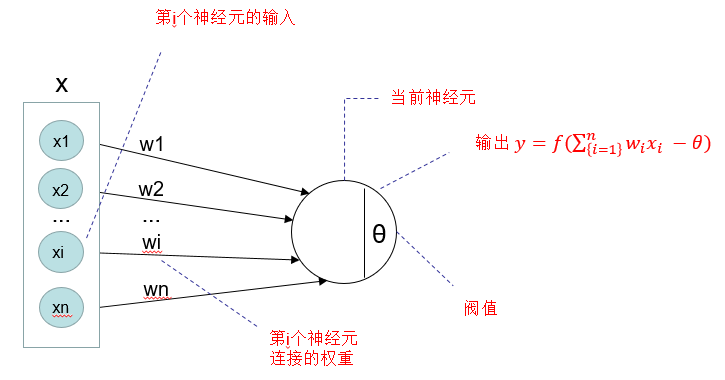
\includegraphics[width=0.95 \textwidth,clip]{nn.png}
	%\hspace{0.02\textwidth}
	%\vspace*{-0.08cm}
    \caption{神经元模型示意图}
	\vspace*{-3.5mm}
	\label{fig:nn-example}
\end{figure}
理想中的激活函数是如公式\ref{eq:activate-sgn},将输入值映射为输出值"1"或者"0",其中"1"对应神经元兴奋,"0"对应于神经元抑制,但是因为该阶跃函数具有不连续、不光滑等性质。因此常采用Sigmoid函数作为激活函数,一般来说激活函数是非线性的、可微的。如果不使用线性激活函数,采用线性激活函数(恒等激活函数,图例中$f(x) = x$)的话,那么神经网络只是把输入线性组合再输出,和没有采用神经网络是一样的。
\begin{equation}\label{eq:activate-sgn}
    sgn(x)=\left\{
    \begin{aligned}
    1, x\geq 0 \\
    0, x<0 \\
    \end{aligned}
    \right.
\end{equation}
例如sigmoid函数可以把$(-\infty,+\infty)$输入值映射到(0,1)区间内。常见的激活函数还有tanh(hyperbolic tangent, tanh)函数、修正线性单元(rectified linear units,ReLU)函数等等。表\ref{tab:activate-func}详细的列出了3个常用激活函数的原函数、一阶导数、以及函数的值域。其中tanh函数只是sigmoid函数向下平移再拉升的结果。并且在实际应用中,tanh的效果是好于sigmoid,因为tanh的函数值域是属于(-1,1)的,使用tanh代替sigmoid,会使得神经元输出的均值趋近于0而不是0.5,这样的结果会使得下一层的学习变得更加简单。但是对于多层的神经网络,sigmoid和tanh在极大或极小时梯度会趋近于0,会造成梯度弥散问题。但是对于ReLU 来说,当小于0时,梯度是小于0的,当大于0是,梯度是常数。ReLU激活函数在实际训练中取得了良好的效果。但是对于小于0的部分,此时的梯度为0,神经元不会训练,因此研究者们提出了LeakyReLU等激活函数解决这一问题。
\begin{table}[htpb]
  \centering
  \caption{常见激活函数的介绍}
  \label{tab:activate-func}
  \begin{tabular}{c|c}
    \toprule
    函数名称~~~ & 原函数 ~~~~~~~~一阶导数$f^{'}(x)$~~~~~~~~原函数值域 \\
    \midrule
    sigmoid函数 & $\sigma(x) = \frac{1}{1+e^{-x}}$ ~~~~~~~ $f^{x}(x)=\sigma(x)(1-\sigma(x))$ ~~~~~~~ (0,1) \\ \\
    tanh函数 & $tanh(x) = \frac{e^x-e^{-x}}{e^x+e^{-x}}$ ~~~~ $f^{'}(x)=1-tanh(x)^{2}$ ~~~~ (-1,1) \\ \\
    ReLU函数 & $relu(x) = max(0,x)$ ~~~~~~~~  $sgn(x)=\left\{ \begin{aligned} 1, x\geq 0 \\ 0, x<0 \\ \end{aligned} \right.$ ~~~~~~~ $ [0,+\infty)$ \\ \\
    \bottomrule
  \end{tabular}
\end{table}

前面介绍了神经元模型和各类激活函数,这里需要提到是深度神经网络、目标函数、优化方法。相比前面的单层神经网络,更常见的如图\ref{fig:mnn-example}所示的包含多个层级结构的神经网络,又称为``多层前馈神经网络''(multi-layer feed forward neural networks),其中神经元同一层之间不存在连接,跨层的神经元之间也不存在连接。就如图\ref{fig:mnn-example}所示,其中输入层的神经元接收外接的输入,隐层与输出层的神经元对输入的数据进行处理,这里的网络包含两个隐藏层(hidden layer)和一个输出层(output layer),假设输入为$x$,那么该网络可以形似化为
$H_{\theta}(x) = f_3(w_{3}f_2(w_{2}(f_{1}(w_{1}x+b_1))+b_2)+b_3)$, 其中$f_{1},f_{2}$分别是隐藏层的激活函数,$f_{3}$是输出层的激活函数。假设对于当前任务的目标函数(object function)如\ref{eq:loss-1},需要最小化目标函数$L_{\mathbf{X},\mathbf{Y}}$的值, 对于训练的过程来说,就是不断接受输入层的$(x,y)$,$y$是样本的标签,随着$x$的不断输入,不断调整网络的连接权重$w_1,w_2,w_3$。 常用的优化算法包括随机梯度下降法(stochastic gradient descent,SGD)来迭代优化连接权重,对于一条样本$x_{i},y_{i}$,其连接权重的更新方法如。
\begin{equation}
    \begin{split}
        w_i  \leftarrow w_i +\bigtriangleup w
    \end{split}
\end{equation}
不同层之间的梯度通过误差逆传播(error Back Propagation 简称BP)\cite{rumelhart1988learning}算法进行整个网络的学习。SGD因为更新比较频繁会造成损失函数动荡,最终停留在局部最小值或鞍点。之后又新衍生出的包括Monmentum、Adagrad\cite{duchi2011adaptive}和Adam\cite{kingma2014adam},这些算法能减少迭代的轮数,训练速度更快的收敛到最优值。
\begin{equation}\label{eq:loss-1}
    L(\mathbf{X},\mathbf{Y}) = \sum_{(x_i,y_i) \in (\mathbf{X},\mathbf{Y})}(y_{i} - H_{x}(x_{i}))
\end{equation}

\begin{figure}[htpb]
	\centering
	%	\includegraphics[width=0.48 \textwidth, trim=10 10 10 80,clip]{./pic/example_new.pdf}
	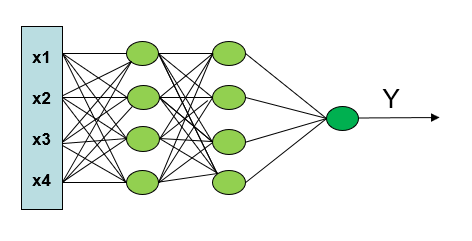
\includegraphics[width=0.80 \textwidth,clip]{multilayer.png}
	%\hspace{0.02\textwidth}
	%\vspace*{-0.08cm}
    \caption{两个隐藏层的神经网络示意图}
	\vspace*{-3.5mm}
	\label{fig:mnn-example}
\end{figure}

%%%%%%%%%%%%%%%%%%%%%%%%%%%   卷积神经网络的介绍   %%%%%%%%%%%%%%%%%%%%%%

\subsubsection{卷积神经网络的介绍}
卷积神经网络(Convolutional Neural Network,CNN)是深度学习的代表算法之一,由LeCun首次实现并且应用。卷积神经网络的主要作用是提取特征,该网络受到生物学的影响,相比较与全连接神经网络,卷积神经网络的主要特性包括局部感知和参数共享。局部感知指对于具有空间特征的输入来说,每个神经元没必要知道全局的信息,只需要感知局部的信息,然后在更高层将局部的信息合并起来得到更高层的信息。对于权值共享来说,每个卷积核与位置无关,因为假设对于图像来说,其中某一部分的统计特性和其它的部分是一样的,所以对于其中的一个卷积核来说,可以应用到图像上的任何地方去。所以,局部感知和参数共享不仅能提取到更多的特征,并且能大幅度减少参数的数量。因此,卷积神经网络广泛的应用在图像、视频、音频和文本等各种模态的数据上,并且都取得了巨大的成功。

卷积神经网络的特征提取层主要包括两个模块,分别是卷积层(convolutional layer)和池化层(pooling layer),两者的顺序,一般是先通过卷积层,然后是池化层。对于卷积层,主要的作用是提取特征,卷积层的核心是卷积核(kernel),其本质还是神经元。但是卷积核的感受野和全连接的神经元是不同的,这里的感受野是局部的,并且感受野的大小由卷积核的大小控制。如图\ref{fig:con-example}所示,当前卷积核的大小是$4 \times 4$的,对于输入的图片$6 \times 6 \times 3$,其中图片输入的3为图片的通道数、$6 \times 6$为高宽,假设滑动的步骤为$1$,卷积核通过在输入图片上按照步长进行滑动并且进行对应位置的点乘运算,最后形成一个$4 \times 4$ 的特征图。以上综合起来就是卷积操作,其中$3 \times 3$就是网络的参数。按照惯例,输入的图片可以有固定的的高宽和通道数时,卷积核可以有不同的高宽,但是必须是固定的通道数,这里一般和输入的通道数一致。有多少个卷积核,最后就能得到多少个特征图(feature map)。
\begin{figure}[htpb]
	\centering
	%	\includegraphics[width=0.48 \textwidth, trim=10 10 10 80,clip]{./pic/example_new.pdf}
	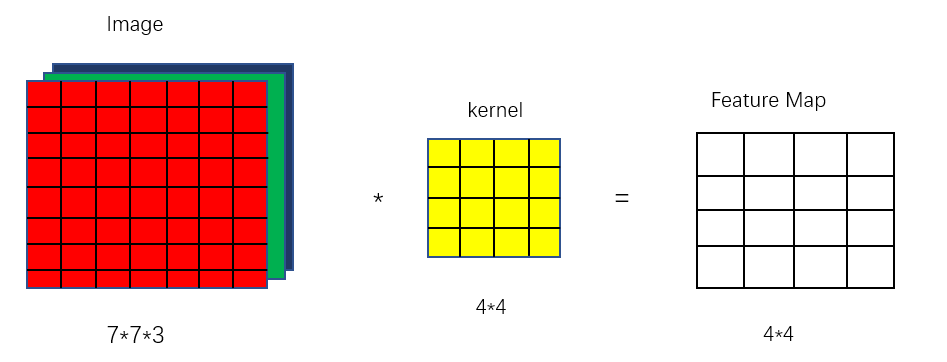
\includegraphics[width=0.95 \textwidth,clip]{conv.png}
	%\hspace{0.02\textwidth}
	%\vspace*{-0.08cm}
    \caption{卷积神经网络的卷积层示意图}
	\vspace*{-3.5mm}
	\label{fig:conv-example}
\end{figure}

对于池化层来说,主要的作用是对于卷积层输出的特征图提取主要特征,降低网络的参数,且有防止过拟合的作用。常见的池化包括平均池化(Average pooling)和和最大池化(Max pooling)。具体细节如图\ref{fig:pooling-example}所示,池化也是通过类似卷积的操作实现的,在图例中,池化也是以$2 \times 2$在特征图上进行滑动,滑动的步骤为$2$,而最大池化是选着窗口中的最大值作为输出,平均池化是选择窗口中所有值的平均值进行输出,假设输入的特征图为$C \times W \times H$ ,那么经过如图例所示的操作后得到的特征图为$C \times \frac{W}{2} \times \frac{H}{2}$。
\begin{figure}[htpb]
	\centering
	%	\includegraphics[width=0.48 \textwidth, trim=10 10 10 80,clip]{./pic/example_new.pdf}
	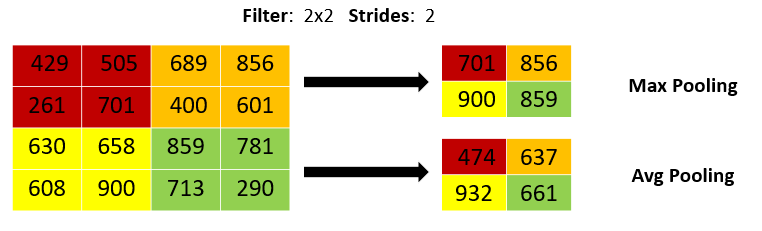
\includegraphics[width=0.95 \textwidth,clip]{pooling.png}
	%\hspace{0.02\textwidth}
	%\vspace*{-0.08cm}
    \caption{卷积神经网络的池化层示意图}
	\vspace*{-3.5mm}
	\label{fig:pooling-example}
\end{figure}

综合上述对于卷积神经网络的卷积和池化的介绍,因为每层的输入和输出都表现为特征图的形式,因此卷积神经网络可以和全连接的网络一样可以有多层,并且取得更好的效果。LeNet-5\cite{lecun1998gradient-based}是
Yang LeCun等人在$1988$年提出的,它是第一个成功应用于数字识别问题的卷积神经网络,在著名的MINIST数据集上,LeNet-5可以取得大约$99.2\%$的准确率。LeNet-5是一个经典的卷积神经网络,前5层分别是卷积层和池化层,后2层全连接层。之后于$2012$ 年提出的AlexNet\cite{krizhevsky2012imagenet},其网络结构如图\ref{fig:alexnet-example}首次使用Relu激活函数替代Sigmoid,并且验证了其在较深网络上的作用,成功解决了Sigmoid在较深网络的梯度弥散问题,虽然Relu 很早就提出了。其次,AlexNet首次在训练中使用dropout层抑制一部分激活的神经元,以避免过拟合,并且通过实践证明了效果。与此同时,模型还采用了数据增强等trick来防止过拟合,使用cuda提高训练速度。而之后提出的VGG\cite{simonyan2015very},相比较与之前的LeNet和AlexNet,最大的特点是网络更深,具有16-19层,不包含池化和最后的softmax层。
\begin{figure}[htpb]
	\centering
	%	\includegraphics[width=0.48 \textwidth, trim=10 10 10 80,clip]{./pic/example_new.pdf}
	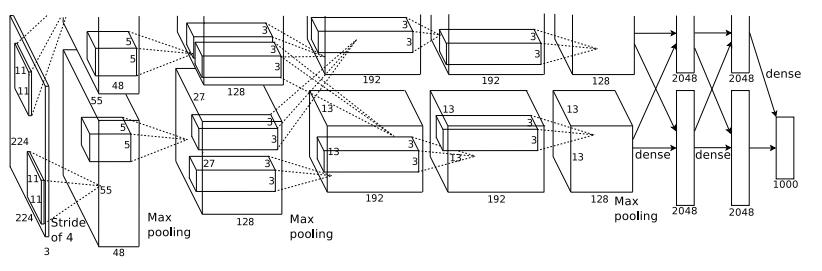
\includegraphics[width=0.95 \textwidth,clip]{alexnet.png}
	%\hspace{0.02\textwidth}
	%\vspace*{-0.08cm}
    \caption{AlexNet网络结构示意图}
	\vspace*{-3.5mm}
	\label{fig:alexnet-example}
\end{figure}
ResNet\cite{he2016deep}是何凯明等人(2016)提出的,针对前面网络并不能随着层数的叠加而性能的提高,ResNet首次提出了残差学习单元。如图\ref{fig:resnet-example}所示,假设模块的输入为$x$,$F(x)$指的是网络中的一系列的张量运算,假设神经网络最优的拟合结果为$H(x) = F(x) + x$,那么神经网络的最优的映射函数$F(x)$为$H(x)$和$x$之间的残差。通过不断的叠加这个模块,可以不断堆叠加深网络的深度但是不降低网络性能。
\begin{figure}[htpb]
	\centering
	%	\includegraphics[width=0.48 \textwidth, trim=10 10 10 80,clip]{./pic/example_new.pdf}
	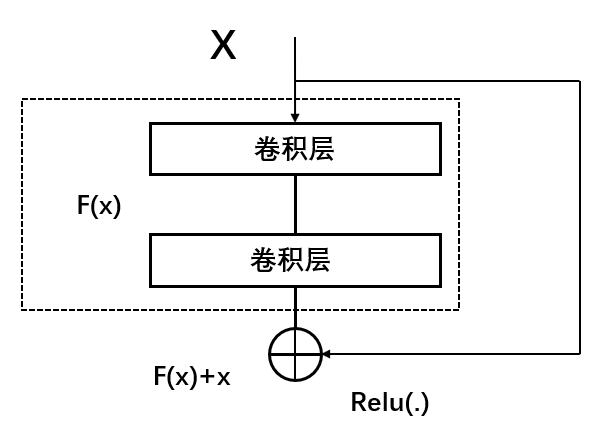
\includegraphics[width=0.75 \textwidth,clip]{resnet.png}
	%\hspace{0.02\textwidth}
	%\vspace*{-0.08cm}
    \caption{ResNet残差学习单元示意图}
	\vspace*{-3.5mm}
	\label{fig:resnet-example}
\end{figure}

综上,卷积神经网络自提出以来,得到了极大的发展,表现为新的激活函数,降低过拟合的dropout层,残差学习模块,加上cuda硬件加速的发展,我们能训练更复杂更深的神经网络,取得更好的性能。

%%%%%%%%%%%%%%%%%%%%%%%%%%%%%%%% 图推理 %%%%%%%%%%%%%%%%%%%%%%%%%%%%%%%%%%%%%%%%%%

\subsection{消息传递}

图推理是消息传递的一种形式,条件随机场(Conditional Random Field)广泛的用在了图推理问题上。Johnson\cite{johnson2015image}将CRF用于图像检索领域的场景图谱与对应图片的绑定的推断。本文用的方法类似于CRFasRNN\cite{zheng2015conditional}和Graph-LSTM\cite{liang2016semantic}。本文的方法是收到\cite{xu2017scene}的启发,Xu在场景图谱的生成任务中,设计了原始图和对偶图,原始图用于图片中物体节点的预测,对偶图用于关系节点的预测。和之前不同的是,我们只是对其中的关系节点构建图,通过关系的消息传播机制,我们的模型是迭代的提纯社会关系理解的预测。而不是像标准的循环神经网络(Recurrent Neural Network)只是单次预测,并不能达到提纯的效果。下面的部分我们介绍关于CRF和本文中用到了循环神经网络(RNN)以及门控循环网络(Gated Recurrent Unit,GRU)。

\subsubsection{条件随机场}
CRF是一种判别式无向图模型,用于对条件分布建模,在给定随机变量\texbf{X}的条件下,构建条件概率模型\textbf{P(Y|X)}。条件随机场的定义如下:设\textbf{X}与\texbf{Y}是随机变量,\textbf{P(Y|X)}是在给定
\textbf{X}的条件下\textbf{Y}的条件概率分布。令G = (V,E)表示一个无向图,V是节点的集合,E是无向边,$Y_{v}$表示与节点v对应的标记向量,$w~v$表示在图中所有与节点v有边连接的所有节点w,
$w \neq v$表示节点v以外的所有节点,如果所有的节点$Y_v$都满足公式\ref{eq-crf}  的马尔科夫性质,那么称(Y,X)为一个条件随机场。
\begin{equation} \label{eq-crf}
    P(Y_{v}|X,Y_w,w \neq v) = P(Y_v|X,Y_w,w~v)
\end{equation}
CRF引入了特征函数(指数函数的形式),对于其中的特例线性链条件随机场,线性链条件随机场如图\ref{fig:crf}。
\begin{figure}[htpb]
	\centering
	%	\includegraphics[width=0.48 \textwidth, trim=10 10 10 80,clip]{./pic/example_new.pdf}
	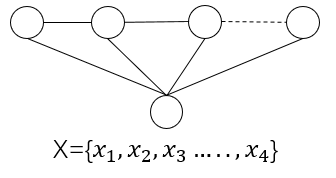
\includegraphics[width=0.75 \textwidth,clip]{crf.png}
	%\hspace{0.02\textwidth}
	%\vspace*{-0.08cm}
    \caption{线性链条件随机场}
	\vspace*{-3.5mm}
	\label{fig:crf}
\end{figure}
其中概率分布如下所示,其中t_{k}和s_{l}都是特征函数,$\lambda_{k}$和$u_{l}$对应的权值。
\begin{equation}
    P(y|x) = \frac{1}{Z}\mathbf{exp}((\sum_{i,k})\lambda_{k}t_{k}(y_{i-1},y_{i},x,i)+\sum_{i,l}\mu_{l}s_{l}(y_{i},x,i))
\end{equation}

\subsubsection{循环神经网路}




\subsection{物体检测与识别}

在社会关系识别的任务中,有一个重要的模块是利用物体识别模型得到人的场景信息,即采用物体识别模型识别去当前图片中包含了哪些物体,得到该物体在图片的区域。物体识别的模型包括Ross等人提出的RCNN\cite{girshick2014rich},fast-RCNN\cite{girshick2015fast},以及Ren等人(2016)\cite{ren2015faster}提出的faster-RCNN。前面提到的三个模型都是基于区域的物体检测模型,RCNN\cite{girshick2014rich} 首次提出在目标图像中有多个目标框,然后判断目标框是否包含物体,具体的检测步骤如下:
(1)其中采用选择性搜索的方法得到图片中的所需要的目标框区域,将得到的区域调整为卷积神经网络输入的消息。
(2)利用一个预训练好的卷积神经网络,提取第一步得到的区域中的特征。
(3)将第二步中得到的特征当作一个线性SVM的输入,得到物体的类别,另外训练一个线性回归模型得到物体的目标框。
RCNN的主要缺点是对于一张图片中的每个感兴趣区域,需要遍历提取其中的特征,然后依次执行物体的分类和物体框的回归,需要耗费较多时间。由于全卷积和池化层不改变某个区域在特征图和原图的位置,因此fast-RCNN 在RCNN 的基础上提出了ROI(region of interest) 池化层,将图片输入到卷积神经网络中,对于特征图上的区域,经过ROI池化层进行调整,然后再继续之后的全连接层和一个线性回归层进行分类和目标框的确定。综上,fast-RCNN 较大程度上提高了物体检测的性能。由于fast-RCNN 在大数据集上的表现依然不能满足实际的需求,因为RCNN和fast-RCNN均采用选择性搜索的方法得到所需要的区域,这个步骤是比较耗费时间。因此faster-RCNN提出RPN(region proposal network),RPN主要网络包括两部分,一部分主要是对生成的anchors进行判断是foreground还是background,其中foreground代表目标,另外一部分主要是对检测框的位置进行调整。经过RPN网络后得到候选区域,再利用ROI池化得到特征向量进行物体类别的判断和物体框的进一步精确判断。

综上,以上的篇幅主要是回顾了在社会关系检测的工作中,有用的物体检测方法和一些相关工作。结论是得益于GPU等硬件设备的发展,物体识别领域的算法也得到了快速的发展,尤其是随着特征提取模块的发展,卷积网络越来越深,能学习到更多更丰富的特征。对于一幅图片,我们能在得到更多的、更准确的物体框和类别。

\section{社会关系检测}
本章将回顾社会关系检测领域的一些相关工作,并且对于消息传递机制的介绍,以及消息传递机制的相关工作的一些介绍。

\subsection{已有工作的简单介绍}

社会关系检测是社交网络的一个基础\cite{li2015celebritynet},社会关系检测作为一个重要的多学科问题,在计算机视觉领域受到越来越多的关注。随着这个问题被提出以来,有大量的工作用于从图片中抽取两个人之间的社会关系。主要有wang 等人(2010)\cite{wang2010seeing},以及Dibeklioglu等人(2013)\cite{dibeklioglu2013like}和Zhang 等人(2015)\cite{zhang2015learning}提出的利用面部表情、年龄、性别、姿势等多种特征的联合模型。Li等人(2017)\cite{li2017dual-glance}提出的多次观察的\textbf{dual-glance}模型。以及Wang 等人(2018)\cite{wang2018deep}提出的基于常识知识的深度推理模型\textbf{GRM}。以及从视频中抽取社会关系的工作ding2010learning等人(2010)、Ramanathan等人 (2013)\cite{ramanathan2013social}。Sun等人(2017)\cite{sun2017a}基于范围的理论,将社会关系划分为5个范围,同时接着这五个范围又划分为16种社会关系并且扩充了PIPA(people in photo album)数据集\cite{zhang2015beyond}。

Zhang~等\cite{zhang2015learning}提出的模型认为从心理学的角度出发,认为人的关系主要由人的面部表情的一些特点决定的。首先,模型设计了一个基准模型用于提取图片中两个人对的特征,对于两个人对,基准模型采用共享参数的深度卷积网络(DCN),利用DCN提取得到的特征分别记为$x^r,x^l$,并且$\forall x^r,x^l \in R^{2048 \times 1}$,经过一个权重矩阵$\mathbf{W} \in R^{4096 \times 256}$得到特征向量$x_t$。对于已经标注好的人脸图片两个人脸分别为和,利用DCN 提取得到的特征分别记为和,并且。除了图片中本来的特征,模型利用了两张人脸在图片的空间信息。1)两张人脸的位置分别表示为${x^l,y^l,w^l,h^l,x^r,y^r,w^r,h^r}$,其中$x-,y-$是左上角的坐标,$w,h$ 分别是两个人脸包围盒的宽度和高度。2)人脸的相对位置$\frac{x^l-x^r}{w^l},\frac{y^l-y^r}{h^l}$。3)人脸之间的比例$\frac{w^l}{w^r}$。以上的三项空间特征会和DCN得到的$x_t$拼接来学习得到关系类别。
\begin{figure}[htpb]
	\centering
	%	\includegraphics[width=0.48 \textwidth, trim=10 10 10 80,clip]{./pic/example_new.pdf}
	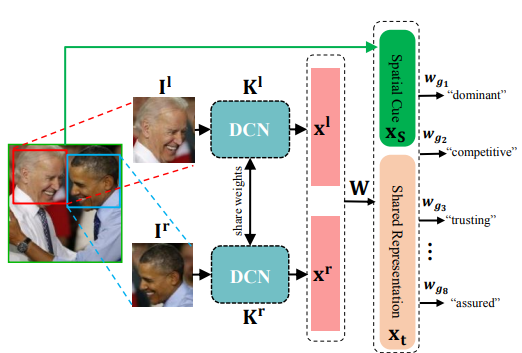
\includegraphics[width=0.75 \textwidth,clip]{1.png}
	%\hspace{0.02\textwidth}
	%\vspace*{-0.08cm}
    \caption{zhang的模型}
	\vspace*{-3.5mm}
	\label{fig:model_zhang}
\end{figure}
\looseness=-1
除此之外,$\mathbf{w_{gi}}$,$\mathbf{W}$,$\mathbf{K^l}$,and $\mathbf{K^r}$可以采用标准的正太分布初始化。结合之前符号的定义,该模型损失函数定义如下:
\begin{equation}
\begin{split}
     arg\max \limits_{\Omega} p({\mathbf{w}_{g_i}}_{i=1}^8, \mathbf{W},\mathbf{K}^r | \mathbf{g},\mathbf{x}_t,\mathbf{x}_s,\mathbf{I}^r,\mathbf{I}^l) \propto \\
     (\sum_{i=1}^{8}p(g_i|x_t,x_s)p(w_(g_i)))(\sum_{j=1}{K}p(k_j^l)p(k_j^r))p(\mathbf(W)), \\
     s.t. \mathbf{K}^r = \mathbf{K}^l
\end{split}
\end{equation}
基于以上的工作,该模型同样认为人的面部属性对最终的关系预测可以起到关键的作用。

Li等人(2017)\cite{li2017dual-glance}基于之前的工作,针对社会检测的任务提出了包含两个关系粒度的数据集,PISC-coarse和PISC-fine(2017)\cite{li2017dual-glance}。该工作首次提出了利用图片中的场景来协助预测两个人之间的关系,场景具体表示为该图片中的物体。直观来说,如果一幅图片中包含电脑桌子等物体,那么大概率是``同事''关系。\textbf{dual-glance}模型分为两个模块,first glance和second glance,first glance 的输入为一张图片$\mathbf{I}$ 和两个人身体的包围盒。针对图片$I$,首先修剪出3个小块,前两个小块分别覆盖住两个人,$p_1$和$p_2$,第三个小块覆盖两个人,表示为$p_{u}$。这三个小块的像素被修正为$224 \times 224$大小,作为后续三个CNNs 网络的输入,其中$p_1$和$p_2$的特征抽取网络是共享网络参数的。此外,包围盒的位置信息对于视觉信息是一种补充,例如亲密关系往往的离得比较近的,无关系的两个人对的包围盒离的较远。位置信息$\mathbf{g}$,经过预训练的ResNet\cite{he2016deep} 抽取得到表示人对关系的特征向量为$v$,经过拼接和全连接网络后得到这个人对的特征向量$v_{top}$。

对于second glance模块,模型利用faster-RCNN\cite{ren2015faster}中的RPN产生一系列的区域候选框$P_{I}$,这些候选框包含物体的概率大于超参数$m$。对于一个人对,我们从集合$P_{I}$ 中选择部分候选框$R(b1,b2;I)$,选择方式如\ref{eq:select-rp},其中函数$G(b1,b2)$表示两个包围盒的IOU,$\tau_{u}$是阀值。
\begin{equation}\label{eq:select-rp}
    R(b1,b2;I) = \{c \in P_{I} : max(G(c,b1),G(c,b2))<\tau_{u}\}
\end{equation}
利用faster-RCNN得到的特征图,采用ROI pooling抽取出固定长度的的向量物体特征向量$v \in R^{k}$。同时用$\{v_i|i=1, 2, .... N\}$作为$R_(v1,b2;I)$中的物体向量集合。然后依次采用公式\ref{eq:atten-1}方式将$v_{top}$和物体的向量集合得到$h_i$。
\begin{equation}\label{eq:atten-1}
    h_i = v_i + w_{top} \otimes v_{top}
\end{equation}
之后采用attention的方式将$h_i$得到最终的得分$s_i$,具体细节如公式\ref{eq:atten-2}所示,其中attention的权重$a_{i} \in [0,1]$
\begin{equation} \label{eq:atten-2}
    \begin{split}
        a_{i} &= \frac{1}{1+exp(-(W_{h,a}h_{i}+b_{a}))} \\
        v^{att}_{i} &= a_{i}v_{i} \\
        s_{i} &= W_{s} v_{i}^{att} + b_{s}
    \end{split}
\end{equation}

\textbf{GRM}(2018)\cite{wang2018deep}同样认为引入当前人对的周边物体的信息对判断人对之间的社会关系是有帮助的,但是现有前面的模型忽略了周边物体的语义和这些物体以及社会关系的先验知识。除此之外,周边物体和社会关系的交互太过简化了。因此,GRM采用深度学习结合先验知识制定了一个图推理模型(Graph Reasoning Model)来实现社会关系检测任务。首先,GRM基于训练集中的样本构建了一个描述物体和社会关系共现的图谱。形式化来说,先验知识图谱表示为$\mathrm{G} = \{\mathrm{V},\mathrm{A}\}$,其中$\mathrm{V}$表示图上的节点集合,$\mathrm{A}$表示节点间的邻接矩阵。当前的图$\mathrm{G}$包含两种节点类型,一种节点表示社会关系,一种表示物体类别,针对当前图片场景构建的图的节点来说,采用相应图片对应区域抽取出的特征向量初始化。对于社会关系节点,这里采用Li等人的方式\cite{li2017dual-glance}的方式修剪出三部分包含人的区域,利用预训练好的ResNet提取出特征向量,与空间信息等特征向量进行拼接得到一个$d$维的特征向量$f_{h},f_{h} \in \mathrm{R}^d$。$f_h$作为所有社会关系节点的初始化向量。对于物体节点来说,我们需要用到在大规模训练集上预先训练好的faster-RCNN\cite{ren2015faster},由于PISC-coarse和PISC-fine等数据集并没有标注好的物体类别。这里的大规模数据集指的是COCO\cite{lin2014microsoft},COCO是专门为了物体识别标注的数据集,包含我们日常生活中常见的80类的物体。利用物体检测模型提取出高于置信度$\phi$($\phi$是一个超参数),对于这里未检测到的物体,采用全$0$的特征向量。
之后利用GGNN(Gated Graph Neural Network)网络\cite{li2016gated}来执行图上的消息传播。通过GGNN,能探索人对和图片场景中物体的交互。物体的类别是一个关键的因素用于区分不同的社会关系,但是由于有的物体的信息对于判定社会关系时不重要的、甚至起到了干扰的作用,因此GRM提出了图注意力的机制,有选择的采用能起到区分不同社会关系的物体节点,按照区分能力的大小给予不同的权重。综上所述,GRM模型提供了一个可解释的方法来提高社会关系检测的能力,从周边场景中推理得到有效的信息。

前文提到了图片上人对的特征和物体的信特征抽取,GRM接下来需要执行不同节点间的信息传播,对于其中GGNN的执行过程,对于图$\mathrm{G}$ 中的节点$v$,其对应的隐藏状态为$h_{v}$,GGNN模型融合邻接节点的信息来更新$v$节点隐藏状态,GGNN采用类似于Gated Recurrent Unit(GRU)\cite{cho2014learning}机制的方式实现节点间的信息融合。所以,对于第$t$步GRU unit的输入为$a_v^t$和$h_v^t$,$a_v^t$是融合邻接物体节点的信息向量,融合方式如公式\ref{eq-aggre},其中$A_v^{\tau}$代表前面提到的物体和社会关系的邻接矩阵,矩阵的值为它们在训练集中共现的概率。
\begin{equation}\label{eq-aggre}
    a_v^t = A_{v}^{\tau}[~h_1^{t-1}~...~h_{|V|}^{t-1}~]^{\tau} + b
\end{equation}
经过$T$此GRU的迭代后,分别得到物体节点、关系节点的隐藏层表示。但是由于周边的物体在区分不同的关系起到不同的作用,GRM采用attention机制来结合物体的信息。attention的如公式\ref{eq:graph-atte},其中得到邻接物体节点权重为$\alpha_{ij}$。进过GGNN、attention两个模块后,得到表示社会关系的特征向量$\mathbf{f}_{i}$,用做最后的分类,取概率最大的作为当前人对的关系。
\begin{equation}\label{eq:graph-atte}
    \begin{split}
        \mathbf{h}_{ij} &= tanh(\mathbf{U}^ah_{r_{i}}) \odot tanh(\mathbf{V}^ah_{o_{j}}) \\
        e_{ij} &= \mathbf{Atten}(\mathbf{h}_{ij}) \\
        \alpha_{ij} &= \sigma(e_{ij})
    \end{split}
\end{equation}

\subsubsection{}







